\subsection{Task 4: Web Server Ở Chế Độ Access Point}
\subsubsection{Wifi}

ESP32 hỗ trợ nhiều chế độ Wi-Fi linh hoạt, cho phép thiết bị hoạt động như một trạm (Station), một điểm truy cập (Access Point), hoặc đồng thời cả hai. Việc chọn đúng chế độ giúp hệ thống phù hợp với từng tình huống triển khai IoT.

\paragraph{Các chế độ Wi-Fi của ESP32}
Để thiết lập chế độ hoạt động Wi-Fi, sử dụng hàm:

\begin{lstlisting}[
	language=C++,
	basicstyle=\ttfamily\small,
	numbers=left,
	numberstyle=\tiny\color{gray},
	numbersep=6pt,
	breaklines=true,
	frame=single,
	rulecolor=\color{blue!60!black},
	backgroundcolor=\color{blue!3}
]
WiFi.mode(...)
\end{lstlisting}

Các chế độ phổ biến:
\begin{itemize}
	\item \texttt{WiFi.mode(WIFI\_STA)}: Chế độ trạm (Station), ESP32 kết nối tới điểm truy cập/router.
	\item \texttt{WiFi.mode(WIFI\_AP)}: Chế độ điểm truy cập (Access Point), các thiết bị khác kết nối trực tiếp tới ESP32.
	\item \texttt{WiFi.mode(WIFI\_AP\_STA)}: Hoạt động đồng thời ở cả hai chế độ AP và STA.
\end{itemize}

\paragraph{Chế độ trạm (Wi-Fi Station)} 
Khi cấu hình ở chế độ \texttt{WIFI\_STA}, ESP32 sẽ kết nối vào mạng Wi-Fi sẵn có (thường là router). Router sẽ cấp địa chỉ IP riêng cho ESP32, từ đó các thiết bị trong cùng mạng có thể giao tiếp với ESP32 thông qua địa chỉ IP này.

\begin{figure}[H]
	\centering
	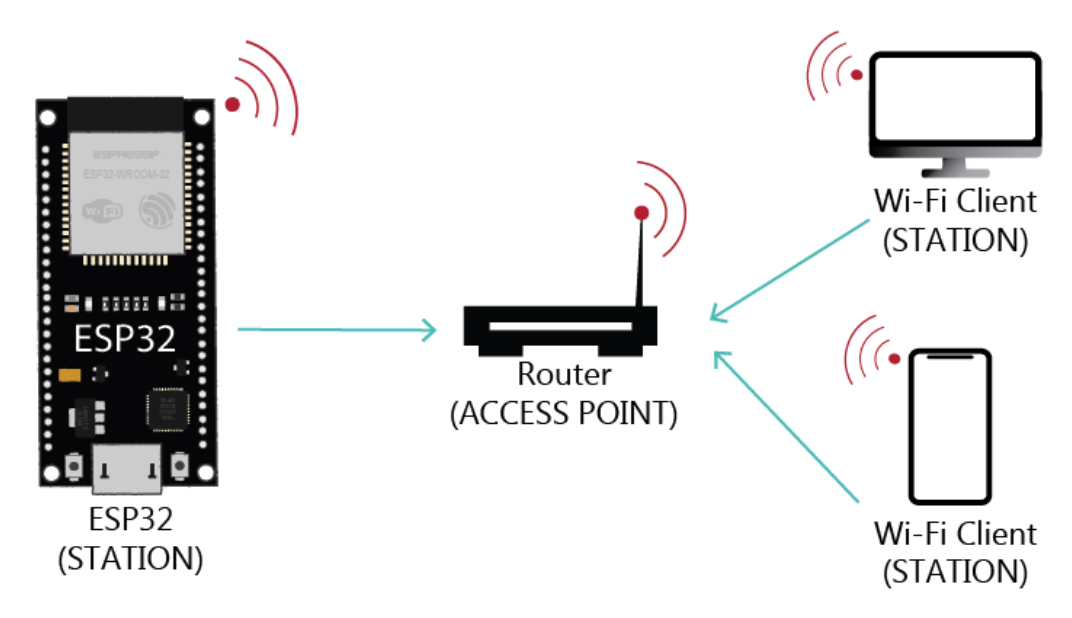
\includegraphics[width=0.8\textwidth]{Pictures/Task4/STA_mode.png}
	\caption{Mô hình kết nối Wi-Fi Station}
	\label{fig:wifi_station_mode}
\end{figure}

Ưu điểm của chế độ này là ESP32 có thể truy cập Internet để:
\begin{itemize}
	\item Gửi hoặc nhận dữ liệu từ API (ví dụ dữ liệu thời tiết).
	\item Đẩy dữ liệu cảm biến lên nền tảng đám mây.
	\item Sử dụng tài nguyên trực tuyến như thư viện JavaScript, biểu tượng, hình ảnh.
\end{itemize}

Tuy nhiên, nếu không có mạng Wi-Fi sẵn có gần đó, chế độ Station sẽ không phù hợp để điều khiển thiết bị cục bộ.

\paragraph{Chế độ điểm truy cập (Access Point)} 
Khi thiết lập \texttt{WIFI\_AP}, ESP32 tự tạo ra một mạng Wi-Fi riêng. Điện thoại, laptop hoặc các thiết bị ESP32 khác có thể kết nối trực tiếp vào mạng này mà không cần router.

\begin{figure}[H]
	\centering
	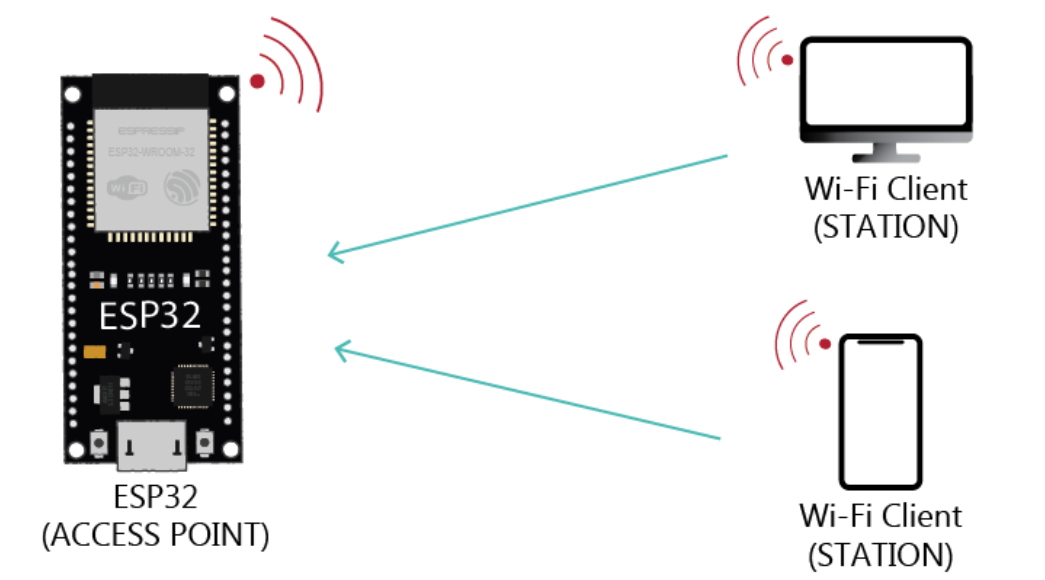
\includegraphics[width=0.8\textwidth]{Pictures/Task4/AP_mode.png}
	\caption{Mô hình kết nối Wi-Fi Access Point}
	\label{fig:wifi_ap_mode}
\end{figure}

Đây là dạng \textit{soft-AP} (điểm truy cập mềm), do đó phù hợp cho giao tiếp cục bộ. Tuy nhiên, vì không đi qua router nên thiết bị kết nối vào soft-AP thường không có Internet, dẫn đến:
\begin{itemize}
	\item Không thể truy cập dịch vụ Internet từ các thiết bị đang nối vào AP của ESP32.
	\item Không phù hợp cho các tác vụ cần HTTP request ra ngoài hoặc đồng bộ cloud trực tiếp qua AP này.
\end{itemize}

Thiết lập cơ bản:
\begin{lstlisting}[
	language=C++,
	basicstyle=\ttfamily\small,
	numbers=left,
	numberstyle=\tiny\color{gray},
	numbersep=6pt,
	breaklines=true,
	frame=single,
	rulecolor=\color{blue!60!black},
	backgroundcolor=\color{blue!3}
]
WiFi.mode(WIFI_AP);
WiFi.softAP(ssid, password);
\end{lstlisting}

Trong đó:
\begin{itemize}
	\item \texttt{ssid}: tên mạng Wi-Fi do ESP32 phát ra (tối đa 63 ký tự).
	\item \texttt{password}: mật khẩu (tối thiểu 8 ký tự), có thể để \texttt{NULL} nếu muốn mạng mở.
\end{itemize}

Hàm \texttt{softAP()} cũng hỗ trợ tham số mở rộng:
\begin{lstlisting}[
	language=C++,
	basicstyle=\ttfamily\small,
	numbers=left,
	numberstyle=\tiny\color{gray},
	numbersep=6pt,
	breaklines=true,
	frame=single,
	rulecolor=\color{blue!60!black},
	backgroundcolor=\color{blue!3}
]
WiFi.softAP(const char* ssid, const char* password,
			int channel, int ssid_hidden, int max_connection)
\end{lstlisting}

Ý nghĩa tham số:
\begin{itemize}
	\item \texttt{channel}: kênh Wi-Fi (1--13).
	\item \texttt{ssid\_hidden}: 0 hiển thị SSID, 1 ẩn SSID.
	\item \texttt{max\_connection}: số thiết bị kết nối đồng thời (1--4).
\end{itemize}

\paragraph{Chế độ kết hợp AP + STA}
ESP32 có thể vừa kết nối đến router, vừa phát Wi-Fi riêng:
\begin{lstlisting}[
	language=C++,
	basicstyle=\ttfamily\small,
	numbers=left,
	numberstyle=\tiny\color{gray},
	numbersep=6pt,
	breaklines=true,
	frame=single,
	rulecolor=\color{blue!60!black},
	backgroundcolor=\color{blue!3}
]
WiFi.mode(WIFI_AP_STA);
\end{lstlisting}
Chế độ này phù hợp cho các ứng dụng cần cấu hình cục bộ qua AP nhưng vẫn duy trì kết nối Internet qua STA.

\paragraph{Quét mạng Wi-Fi lân cận}
ESP32 có thể quét các mạng trong vùng phủ sóng để kiểm tra tín hiệu hoặc xác nhận router có nằm trong phạm vi hoạt động hay không.

Hàm quét:
\begin{lstlisting}[
	language=C++,
	basicstyle=\ttfamily\small,
	numbers=left,
	numberstyle=\tiny\color{gray},
	numbersep=6pt,
	breaklines=true,
	frame=single,
	rulecolor=\color{blue!60!black},
	backgroundcolor=\color{blue!3}
]
int n = WiFi.scanNetworks();
\end{lstlisting}

Sau khi quét, có thể truy xuất thông tin từng mạng:
\begin{itemize}
	\item \texttt{WiFi.SSID(i)}: tên mạng (SSID).
	\item \texttt{WiFi.RSSI(i)}: cường độ tín hiệu thu được (RSSI).
	\item \texttt{WiFi.encryptionType(i)}: kiểu mã hóa mạng.
\end{itemize}

Các kiểu mã hóa thường gặp:
\begin{itemize}
	\item \texttt{WIFI\_AUTH\_OPEN}
	\item \texttt{WIFI\_AUTH\_WEP}
	\item \texttt{WIFI\_AUTH\_WPA\_PSK}
	\item \texttt{WIFI\_AUTH\_WPA2\_PSK}
	\item \texttt{WIFI\_AUTH\_WPA\_WPA2\_PSK}
	\item \texttt{WIFI\_AUTH\_WPA2\_ENTERPRISE}
\end{itemize}

Thông tin RSSI rất hữu ích khi đánh giá nguyên nhân mất kết nối do tín hiệu yếu, từ đó tối ưu vị trí đặt thiết bị hoặc cấu hình anten.

\paragraph{Kết nối ESP32 với mạng Wi-Fi cụ thể}
Để ESP32 kết nối vào một mạng Wi-Fi cụ thể, cần biết trước \texttt{SSID} và \texttt{password} của mạng đó. Ngoài ra, mạng phải nằm trong vùng phủ sóng của ESP32 (có thể kiểm tra trước bằng chức năng quét mạng).

Khai báo thông tin mạng:
\begin{lstlisting}[
	language=C++,
	basicstyle=\ttfamily\small,
	numbers=left,
	numberstyle=\tiny\color{gray},
	numbersep=6pt,
	breaklines=true,
	frame=single,
	rulecolor=\color{blue!60!black},
	backgroundcolor=\color{blue!3}
]
// Replace with your network credentials
const char* ssid = "REPLACE_WITH_YOUR_SSID";
const char* password = "REPLACE_WITH_YOUR_PASSWORD";
\end{lstlisting}

Hàm khởi tạo kết nối Wi-Fi:
\begin{lstlisting}[
	language=C++,
	basicstyle=\ttfamily\small,
	numbers=left,
	numberstyle=\tiny\color{gray},
	numbersep=6pt,
	breaklines=true,
	frame=single,
	rulecolor=\color{blue!60!black},
	backgroundcolor=\color{blue!3}
]
void initWiFi() {
  WiFi.mode(WIFI_STA);
  WiFi.begin(ssid, password);
  Serial.print("Connecting to WiFi ..");
  while (WiFi.status() != WL_CONNECTED) {
    Serial.print('.');
    delay(1000);
  }
  Serial.println(WiFi.localIP());
}
\end{lstlisting}

Sau đó gọi hàm \texttt{initWiFi()} trong \texttt{setup()} để thực hiện kết nối khi thiết bị khởi động.

\paragraph{Nguyên lý hoạt động của hàm kết nối}
\begin{itemize}
	\item \texttt{WiFi.mode(WIFI\_STA)}: đưa ESP32 về chế độ trạm để kết nối vào Access Point/router.
	\item \texttt{WiFi.begin(ssid, password)}: bắt đầu quá trình xác thực và kết nối tới mạng đã chỉ định.
	\item \texttt{while (WiFi.status() != WL\_CONNECTED)}: lặp chờ cho đến khi kết nối thành công.
	\item \texttt{WiFi.localIP()}: lấy địa chỉ IP do router cấp sau khi kết nối thành công.
\end{itemize}

\paragraph{Kiểm tra trạng thái kết nối Wi-Fi}
Hàm \texttt{WiFi.status()} trả về trạng thái kết nối hiện tại. Bảng dưới đây mô tả các giá trị thường dùng:

\begin{table}[H]
	\centering
	\caption{Các trạng thái kết nối Wi-Fi của ESP32}
	\label{tab:wifi_status_codes}
	\begin{tabular}{|c|l|p{7.5cm}|}
		\hline
		\textbf{Giá trị} & \textbf{Hằng số} & \textbf{Ý nghĩa} \\
		\hline
		0 & \texttt{WL\_IDLE\_STATUS} & Trạng thái tạm thời khi vừa gọi \texttt{WiFi.begin()}. \\
		\hline
		1 & \texttt{WL\_NO\_SSID\_AVAIL} & Không tìm thấy SSID phù hợp. \\
		\hline
		2 & \texttt{WL\_SCAN\_COMPLETED} & Quá trình quét mạng đã hoàn tất. \\
		\hline
		3 & \texttt{WL\_CONNECTED} & Kết nối Wi-Fi thành công. \\
		\hline
		4 & \texttt{WL\_CONNECT\_FAILED} & Kết nối thất bại sau các lần thử. \\
		\hline
		5 & \texttt{WL\_CONNECTION\_LOST} & Kết nối đã bị mất. \\
		\hline
		6 & \texttt{WL\_DISCONNECTED} & Thiết bị đang không kết nối mạng Wi-Fi. \\
		\hline
	\end{tabular}
\end{table}

\paragraph{Ngắt kết nối và kết nối lại Wi-Fi}
Để ngắt mạng đã kết nối trước đó, sử dụng:
\begin{lstlisting}[
	language=C++,
	basicstyle=\ttfamily\small,
	numbers=left,
	numberstyle=\tiny\color{gray},
	numbersep=6pt,
	breaklines=true,
	frame=single,
	rulecolor=\color{blue!60!black},
	backgroundcolor=\color{blue!3}
]
WiFi.disconnect();
\end{lstlisting}

\begin{figure}[H]
	\centering
	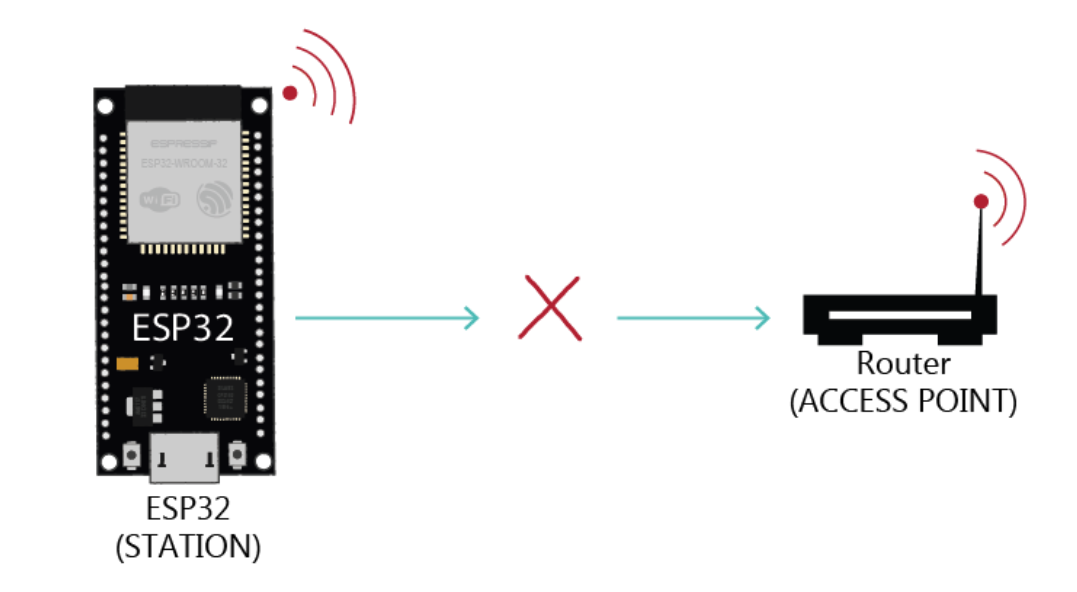
\includegraphics[width=0.8\textwidth]{Pictures/Task4/Disconnected.png}
	\caption{ESP32 đã ngắt kết nối Wi-Fi}
	\label{fig:wifi_disconnect}
\end{figure}

Để thử kết nối lại tới AP đã dùng trước đó:
\begin{lstlisting}[
	language=C++,
	basicstyle=\ttfamily\small,
	numbers=left,
	numberstyle=\tiny\color{gray},
	numbersep=6pt,
	breaklines=true,
	frame=single,
	rulecolor=\color{blue!60!black},
	backgroundcolor=\color{blue!3}
]
WiFi.reconnect();
\end{lstlisting}

Hoặc ngắt rồi kết nối lại bằng \texttt{SSID/password}:
\begin{lstlisting}[
	language=C++,
	basicstyle=\ttfamily\small,
	numbers=left,
	numberstyle=\tiny\color{gray},
	numbersep=6pt,
	breaklines=true,
	frame=single,
	rulecolor=\color{blue!60!black},
	backgroundcolor=\color{blue!3}
]
WiFi.disconnect();
WiFi.begin(ssid, password);
\end{lstlisting}

Trong các hệ thống IoT chạy dài hạn, nên kiểm tra định kỳ và tự động reconnect:
\begin{lstlisting}[
	language=C++,
	basicstyle=\ttfamily\small,
	numbers=left,
	numberstyle=\tiny\color{gray},
	numbersep=6pt,
	breaklines=true,
	frame=single,
	rulecolor=\color{blue!60!black},
	backgroundcolor=\color{blue!3}
]
unsigned long previousMillis = 0;
unsigned long interval = 30000;

void loop() {
  unsigned long currentMillis = millis();
  // if WiFi is down, try reconnecting
  if ((WiFi.status() != WL_CONNECTED) && (currentMillis - previousMillis >= interval)) {
    Serial.print(millis());
    Serial.println(" Reconnecting to WiFi...");
    WiFi.disconnect();
    WiFi.reconnect();
    previousMillis = currentMillis;
  }
}
\end{lstlisting}

\paragraph{Sự kiện Wi-Fi trên ESP32}
ESP32 có thể phát sinh nhiều sự kiện liên quan đến Wi-Fi và Ethernet. Bảng sau tổng hợp các sự kiện thường gặp:

\begin{table}[H]
	\centering
	\caption{Danh sách sự kiện Wi-Fi/Ethernet của ESP32}
	\label{tab:esp32_wifi_events}
	\begin{tabular}{|c|l|p{7.2cm}|}
		\hline
		\textbf{ID} & \textbf{Hằng số sự kiện} & \textbf{Ý nghĩa} \\
		\hline
		0 & \texttt{ARDUINO\_EVENT\_WIFI\_READY} & ESP32 sẵn sàng kết nối Wi-Fi. \\
		\hline
		1 & \texttt{ARDUINO\_EVENT\_WIFI\_SCAN\_DONE} & Hoàn tất quét các điểm truy cập (AP). \\
		\hline
		2 & \texttt{ARDUINO\_EVENT\_WIFI\_STA\_START} & Khởi động trạm (STA). \\
		\hline
		3 & \texttt{ARDUINO\_EVENT\_WIFI\_STA\_STOP} & Dừng trạm (STA). \\
		\hline
		4 & \texttt{ARDUINO\_EVENT\_WIFI\_STA\_CONNECTED} & Trạm ESP32 đã kết nối AP. \\
		\hline
		5 & \texttt{ARDUINO\_EVENT\_WIFI\_STA\_DISCONNECTED} & Trạm ESP32 bị ngắt khỏi AP. \\
		\hline
		6 & \texttt{ARDUINO\_EVENT\_WIFI\_STA\_AUTHMODE\_CHANGE} & Chế độ xác thực của AP đã thay đổi. \\
		\hline
		7 & \texttt{ARDUINO\_EVENT\_WIFI\_STA\_GOT\_IP} & Trạm ESP32 nhận địa chỉ IPv4. \\
		\hline
		8 & \texttt{ARDUINO\_EVENT\_WIFI\_STA\_LOST\_IP} & Trạm ESP32 bị mất địa chỉ IP. \\
		\hline
		9 & \texttt{ARDUINO\_EVENT\_WPS\_ER\_SUCCESS} & WPS ở chế độ đăng ký thành công. \\
		\hline
		10 & \texttt{ARDUINO\_EVENT\_WPS\_ER\_FAILED} & WPS lỗi ở chế độ đăng ký. \\
		\hline
		11 & \texttt{ARDUINO\_EVENT\_WPS\_ER\_TIMEOUT} & WPS hết thời gian chờ ở chế độ đăng ký. \\
		\hline
		12 & \texttt{ARDUINO\_EVENT\_WPS\_ER\_PIN} & WPS nhận mã PIN ở chế độ đăng ký. \\
		\hline
		13 & \texttt{ARDUINO\_EVENT\_WIFI\_AP\_START} & Khởi động soft-AP. \\
		\hline
		14 & \texttt{ARDUINO\_EVENT\_WIFI\_AP\_STOP} & Dừng soft-AP. \\
		\hline
		15 & \texttt{ARDUINO\_EVENT\_WIFI\_AP\_STACONNECTED} & Có thiết bị trạm kết nối vào soft-AP. \\
		\hline
		16 & \texttt{ARDUINO\_EVENT\_WIFI\_AP\_STADISCONNECTED} & Một thiết bị trạm ngắt khỏi soft-AP. \\
		\hline
		17 & \texttt{ARDUINO\_EVENT\_WIFI\_AP\_STAIPASSIGNED} & Soft-AP gán IP cho trạm kết nối. \\
		\hline
		18 & \texttt{ARDUINO\_EVENT\_WIFI\_AP\_PROBEREQRECVED} & Nhận gói probe request ở giao diện soft-AP. \\
		\hline
		19 & \texttt{ARDUINO\_EVENT\_WIFI\_AP\_GOT\_IP6} & Soft-AP nhận địa chỉ IPv6 ưu tiên. \\
		\hline
		19 & \texttt{ARDUINO\_EVENT\_WIFI\_STA\_GOT\_IP6} & Trạm (STA) nhận địa chỉ IPv6 ưu tiên. \\
		\hline
		19 & \texttt{ARDUINO\_EVENT\_ETH\_GOT\_IP6} & Ethernet nhận địa chỉ IPv6 ưu tiên. \\
		\hline
		20 & \texttt{ARDUINO\_EVENT\_ETH\_START} & Khởi động Ethernet ESP32. \\
		\hline
		21 & \texttt{ARDUINO\_EVENT\_ETH\_STOP} & Dừng Ethernet ESP32. \\
		\hline
		22 & \texttt{ARDUINO\_EVENT\_ETH\_CONNECTED} & Ethernet đã kết nối vật lý. \\
		\hline
		23 & \texttt{ARDUINO\_EVENT\_ETH\_DISCONNECTED} & Ethernet bị ngắt kết nối vật lý. \\
		\hline
		24 & \texttt{ARDUINO\_EVENT\_ETH\_GOT\_IP} & Ethernet nhận địa chỉ IPv4. \\
		\hline
		25 & \texttt{ARDUINO\_EVENT\_MAX} & Giá trị giới hạn tối đa cho enum sự kiện. \\
		\hline
	\end{tabular}
\end{table}



\subsubsection{Webserver}



\subsubsection{Triển khai và Code}
